
\documentclass[12pt,a4paper]{scrartcl}

\usepackage[a4paper, left=2cm, right=1cm, bottom=1cm, top=1cm, includeheadfoot]{geometry}
\usepackage[ngerman]{babel}
\usepackage[utf8]{inputenc} % comment this if you uncomment utf8x
%\usepackage[utf8x]{inputenc} % uncomment this if there are problems with 'ä', 'ü', 'ö'
\usepackage{ucs}
\usepackage[usenames,dvipsnames]{xcolor}
\usepackage[fleqn]{amsmath}
\usepackage{amsfonts}
\usepackage{amssymb}
\usepackage{color}
\usepackage{listings}
\usepackage{hyperref}
\usepackage{amsfonts}
\usepackage{listings}
\usepackage{scrpage2}
\usepackage{graphicx}


\definecolor{mygray}{rgb}{0.9,0.9,0.9}
\lstset{language=[Visual]Basic, morekeywords={param, local}}


\lstset{
   literate={ö}{{\"o}}1
           {ä}{{\"a}}1
           {ü}{{\"u}}1
           {ß}{{\ss}}1
           {é}{{\'e}}1,
   inputencoding=ansinew,
   extendedchars=true,
   basicstyle=\scriptsize\ttfamily,
   numberstyle=\scriptsize,
   breaklines=true,
   tabsize=2,
   numbersep=5pt
}
\lstdefinestyle{customcpp}{
   language=C++,
   backgroundcolor=\color{mygray},
   numbers=left,
   keywordstyle=\color{blue}\bfseries,
   stringstyle=\color{BrickRed}\ttfamily,
   commentstyle=\color{OliveGreen}\ttfamily,
   showspaces=false,
   showstringspaces=false,
   showtabs=false
}
\lstdefinestyle{customoutput}{
   backgroundcolor=\color{mygray},
   numbers=none,
   showspaces=false,
   showtabs=false
}

\newcommand{\sourceCode}[1]{\lstinputlisting[style=customcpp]{#1}} %beinhaltet alle benötigten Packages etc.
\begin{document}
\graphicspath{{./}}

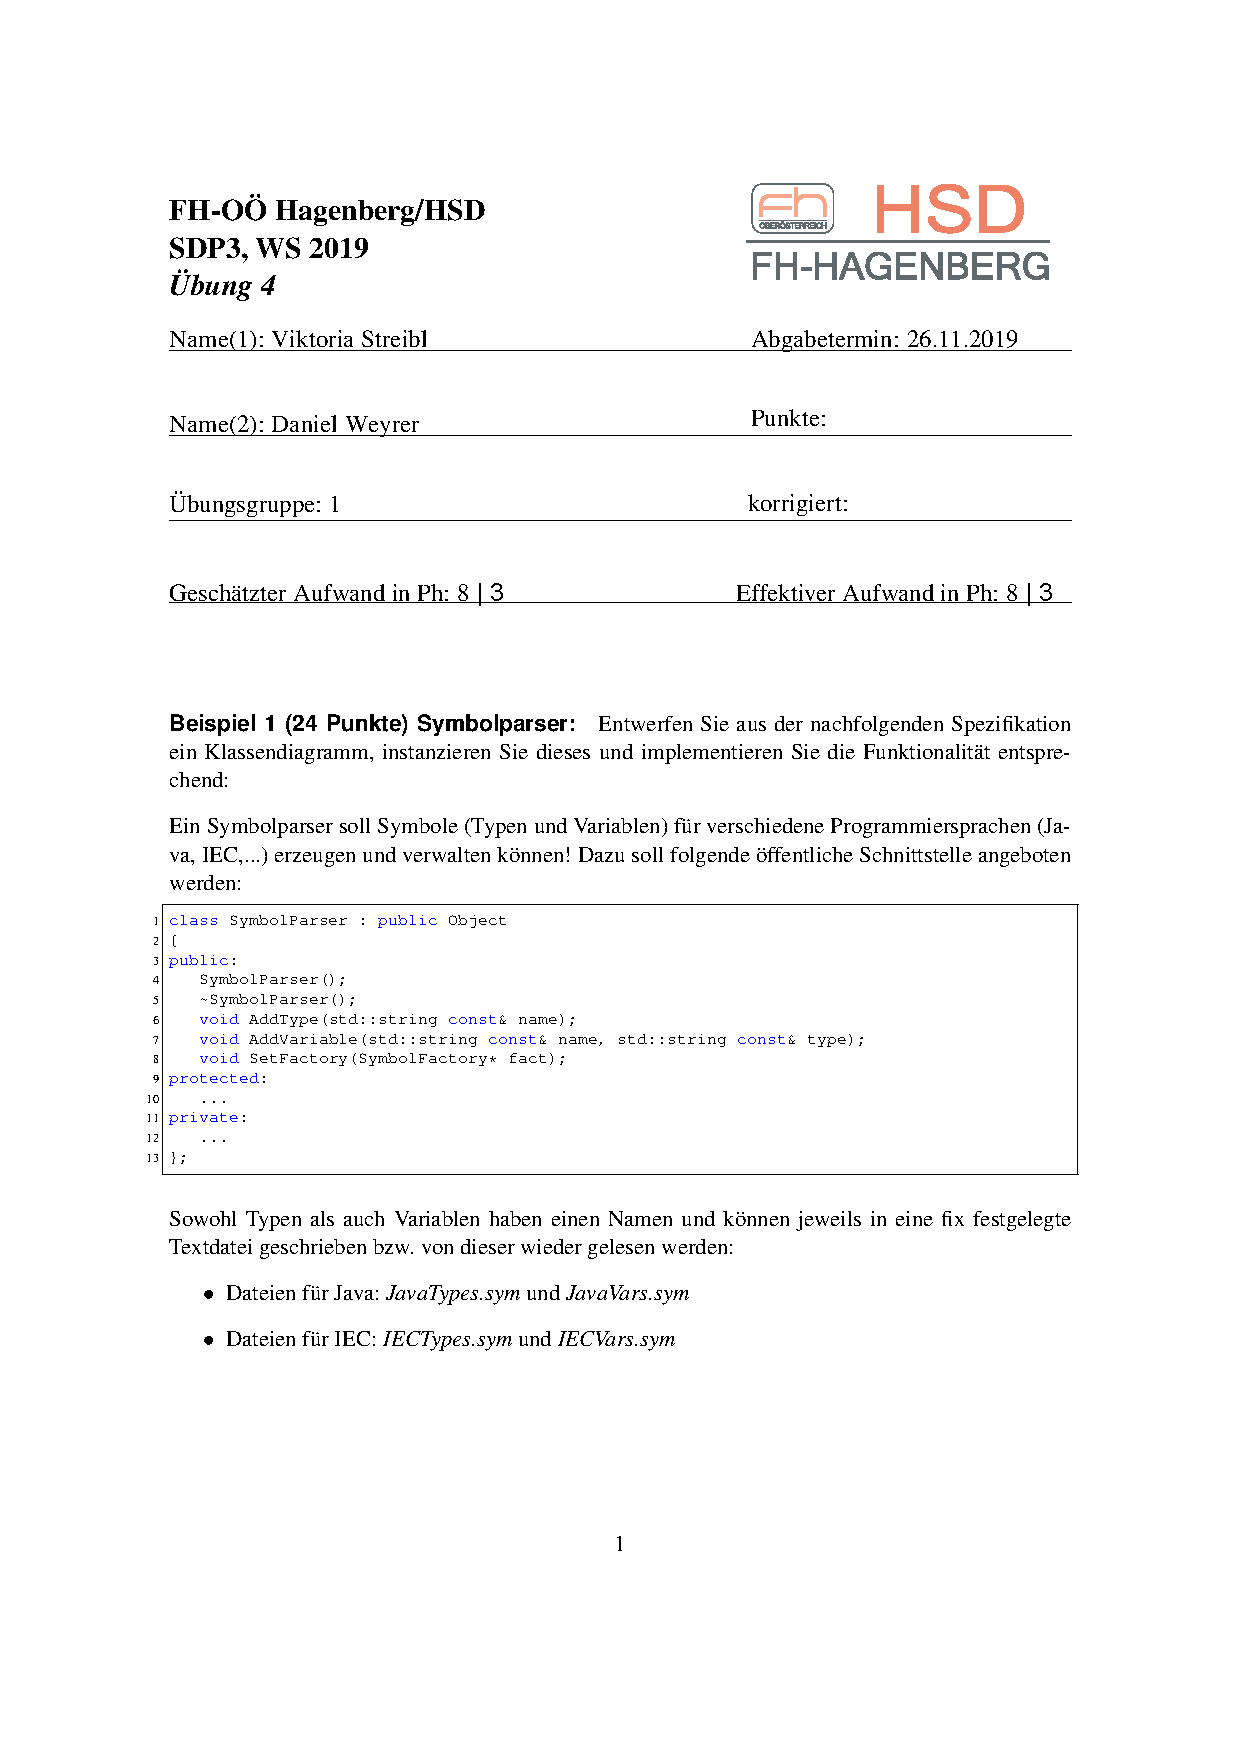
\includepdf[pages=-]{Angabe.pdf}

\title{SDP - Exercise 04} % Übungsname und Nummer angeben
\subtitle{winter semester 2019/20} % Semester angeben oder auskommentieren, falls nicht erwünscht
\author{
Viktoria Streibl - S1810306013\\
  Daniel Weyrer - S1820306044
} % Autorenname
\date{\today} % Das heutige Datum automatisch einfügen

\maketitle % Titelseite erstellen

\newpage
\tableofcontents % Inhaltsverzeichnis erstellen
\newpage

\ihead{Viktoria Streibl}
\ohead{Daniel Weyrer}
\chead{SDP3-UE Uebung 04}

\section{Organizational}
\subsection{Team}
\begin{itemize}
	\item Viktoria 	Streibl 		- 	S1810306013
	\item Daniel 	Weyrer		-	S1820306044
\end{itemize}

\subsection{Roles and responsibilities}
\subsubsection{Jointly}
\begin{itemize}
	\item Planning
	\item Documentation
	\item Systemdocumentation
	\item Class Diagram
\end{itemize}

\subsubsection{Viktoria Streibl}
\begin{itemize}
	\item Class SymbolParser
	\item Class SymbolFactory
	\item Class IECSymbolFactory
	\item Class JavaSymbolFactory
	
	\item TestDriver	
	
	\item Documentation	
\end{itemize}

\subsubsection{Daniel Weyrer}
\begin{itemize}
	\item Documentation
\end{itemize}

\subsection{Effort}

\subsubsection {Viktoria Streibl}
\begin{itemize}
	\item estimated: 6 ph 
	\item actually: 6 ph
\end{itemize}

\subsubsection {Daniel Weyrer}
\begin{itemize}
	\item estimated: 3 ph 
	\item actually: 3 ph
\end{itemize}

\section{Requirenment Definition(System Specification)}


\section{System Design}
\subsection{Classdiagram}
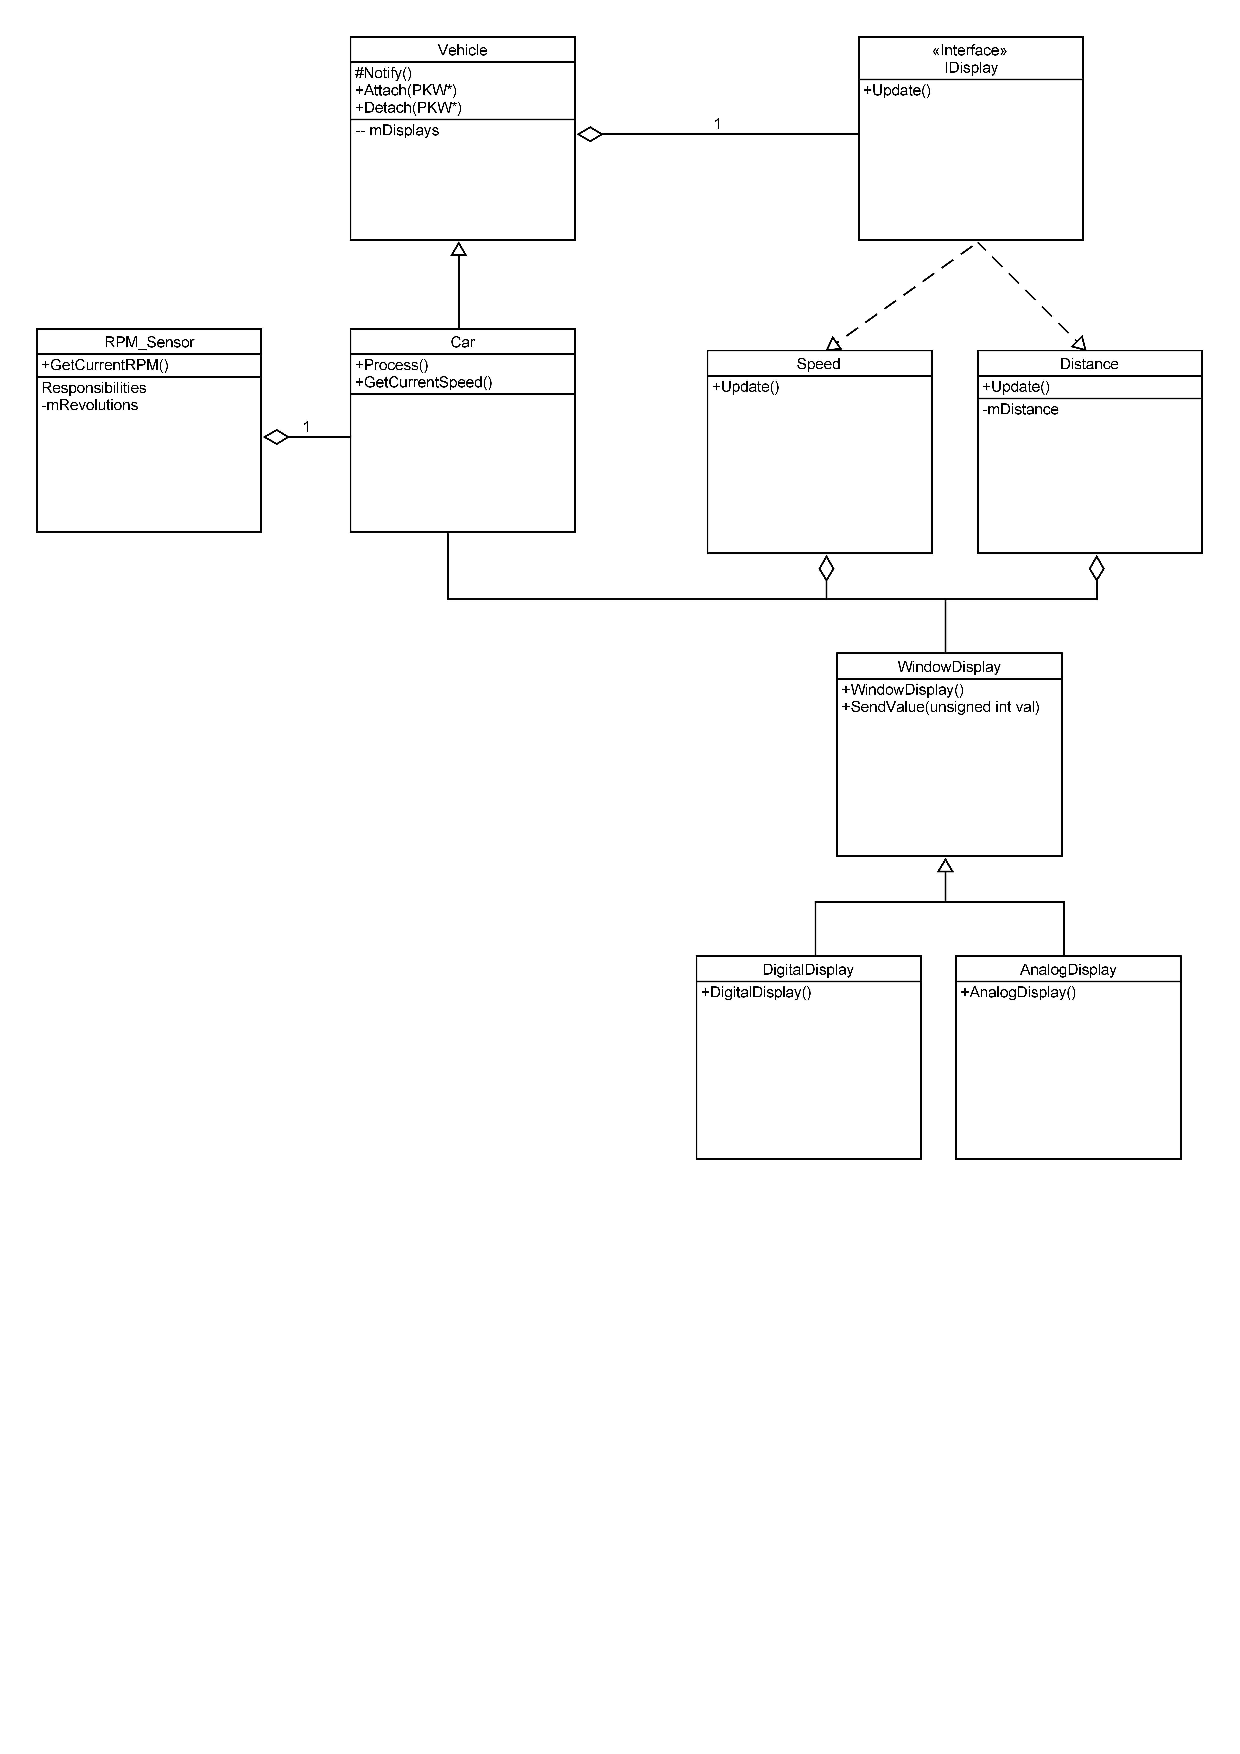
\includegraphics[scale=0.56, angle=90]{ClassDiagramm}

\subsection{Design Decisions}
\subsubsection{}
	
\section{Component Design}
\subsection{SymbolParser}




\subsection{SymbolFactory}

\subsection{IECSymbolFactory}
\subsubsection{WriteIntoFile}
Opens the Type and Variable file and writes every single type and variable into the file by iterating through both vectors.

\subsubsection{ReadFromFile}
Opens the File, reads the content into an ifstream before it gets converted to an string. The string gets handed over to the specific function till it reaches EOF.
This get`s done for both of the files in the object (Variables and Types).

\subsection{JavaSymbolFactory}
\subsubsection{WriteIntoFile}
Opens the Type and Variable file and writes every single type and variable into the file by iterating through both vectors.

\subsubsection{ReadFromFile}
Opens the File, reads the content into an ifstream before it gets converted to an string. The string gets handed over to the specific function till it reaches EOF.
This get`s done for both of the files in the object (Variables and Types).


\subsection{TestDriver}
The Testdriver test alle functions of the clients. It tests the interface for the Epos-Company as well as the NortelNetwork-Company. It encrypt and decrypt several files. It contains also some functions:
\begin{itemize}
\item int main()
\subitem It calls all tests.

\item void CreateFullTest(subtitle, filename)
\subitem This function calls the function to print the title of the tests. Then i tests the Epos functionality and the Nortel Network functionality.

\item void testEPOS(fileName)
\subitem It calls at first the encrypting method of the specific file and than the decrypting method.

\item void testNN(type, fileName)
\subitem It calls at first the encrypting method of the specific file tests all encoding types, than it decrypts the outcome.

\item void PrintSubheader(subtitle)
\subitem This function outputs the title of the following test.
\end{itemize}
Following tests are implemented:
\begin{itemize}
\item Test alphabet and numbers
\item Test special characters
\item Testing an email file
\item Test if no file is there
\item Test if file is empty
\end{itemize}
It ouputs a error message if there was no successful run.

\newpage
\section{Test Protocol}

\subsection{Testfiles}




\newpage
\section{Source Code}

\subsection{SymbolParser}
\subsubsection{SymbolParser.h}
\sourceCode{./SymbolParser/SymbolParser/SymbolParser.h}
\subsubsection{SymbolParser.cpp}
\sourceCode{./SymbolParser/SymbolParser/SymbolParser.cpp}
\newpage

\subsection{SymbolFactory}
\subsubsection{SymbolFactory.h}
\sourceCode{./SymbolParser/SymbolParser/SymbolFactory.h}
\subsubsection{SymbolFactory.cpp}
\sourceCode{./SymbolParser/SymbolParser/SymbolFactory.h}
\newpage

\subsection{IECSymbolFactory}
\subsubsection{IECSymbolFactory.h}
\sourceCode{./SymbolParser/SymbolParser/IECSymbolFactory.h}
\subsubsection{SymbolFactory.cpp}
\sourceCode{./SymbolParser/SymbolParser/IECSymbolFactory.h}
\newpage

\subsection{JavaSymbolFactory}
\subsubsection{JavaSymbolFactory.h}
\sourceCode{./SymbolParser/SymbolParser/JavaSymbolFactory.h}
\subsubsection{JavaSymbolFactory.cpp}
\sourceCode{./SymbolParser/SymbolParser/JavaSymbolFactory.h}
\newpage



\subsection{TestDriver}
\subsubsection{TestDriver.cpp}
\sourceCode{./SymbolParser/SymbolParser/TestDriver.cpp}
\newpage
% Um Quellcode einzufügen einfach diesen Befehl verwenden:
%\sourceCode{Relativer/Pfad/zum/SourceCode.Endung}

\end{document}